% !TEX TS-program = pdflatex
% !TEX encoding = UTF-8 Unicode

% This file is a template using the "beamer" package to create slides for a talk or presentation
% - Giving a talk on some subject.
% - The talk is between 15min and 45min long.
% - Style is ornate.

% MODIFIED by Jonathan Kew, 2008-07-06
% The header comments and encoding in this file were modified for inclusion with TeXworks.
% The content is otherwise unchanged from the original distributed with the beamer package.

\documentclass[handout]{beamer}
\usepackage{pgfpages}
\usepackage{amsmath,tikz,tkz-euclide}
\usetkzobj{all}
%\pgfpagesuselayout{4 on 1}[a4paper,border shrink=5mm]

% Copyright 2004 by Till Tantau <tantau@users.sourceforge.net>.
%
% In principle, this file can be redistributed and/or modified under
% the terms of the GNU Public License, version 2.
%
% However, this file is supposed to be a template to be modified
% for your own needs. For this reason, if you use this file as a
% template and not specifically distribute it as part of a another
% package/program, I grant the extra permission to freely copy and
% modify this file as you see fit and even to delete this copyright
% notice. 


\mode<presentation>
{
  \usetheme{Warsaw}
  % or ...

  \setbeamercovered{transparent}
  % or whatever (possibly just delete it)
}


\usepackage[english]{babel}
% or whatever

\usepackage[utf8]{inputenc}
% or whatever

\usepackage{times}
\usepackage[T1]{fontenc}
% Or whatever. Note that the encoding and the font should match. If T1
% does not look nice, try deleting the line with the fontenc.

%%% MATH RELATED
\usepackage{amsmath,amsthm,amssymb}
\usepackage{mathrsfs}  
\usepackage[all]{xy}
\newcommand{\bbc}{\mathbb{C}}
\newcommand{\bbr}{\mathbb{R}}
\newcommand{\bbn}{\mathbb{N}}
\newcommand{\M}{\mathscr{M}}
\renewcommand{\L}{\mathcal{L}}
\newcommand{\vocab}[1]{\textbf{#1}}
\newcommand{\Bis}{\text{Bis}}
\newcommand{\spec}{\text{spec}}
\newcommand{\ol}[1]{\overline{#1}}
\newcommand{\wt}[1]{\widetilde{#1}}
\newcommand{\Ad}{\textnormal{Ad}}

\theoremstyle{definition}
\newtheorem{defn}{Definition}
\newtheorem{quest}{Question}
\newtheorem{prob}{Problem}
\newtheorem{obs}{Observation}
\newtheorem{ex}{Example}
\newtheorem{notation}{Notation}
\newtheorem{thm}{Theorem}
\newtheorem{prop}{Proposition}
\newtheorem{cor}{Corollary}

\title{Math Competition Questions 4}

\subtitle
{Math 180 Strategies of Problem Solving}

\author[W.R. Casper] % (optional, use only with lots of authors)
{}%{W.R. Casper}
% - Use the \inst{?} command only if the authors have different
%   affiliation.

\institute[California State University Fullerton] % (optional, but mostly needed)
{
  Department of Mathematics\\
  California State University Fullerton}
% - Use the \inst command only if there are several affiliations.
% - Keep it simple, no one is interested in your street address.

\subject{Talks}
% This is only inserted into the PDF information catalog. Can be left
% out. 



% If you have a file called "university-logo-filename.xxx", where xxx
% is a graphic format that can be processed by latex or pdflatex,
% resp., then you can add a logo as follows:

% \pgfdeclareimage[height=0.5cm]{university-logo}{university-logo-filename}
% \logo{\pgfuseimage{university-logo}}



% Delete this, if you do not want the table of contents to pop up at
% the beginning of each subsection:
\AtBeginSubsection[]
{
  \begin{frame}<beamer>{Outline}
    \tableofcontents[currentsection,currentsubsection]
  \end{frame}
}


% If you wish to uncover everything in a step-wise fashion, uncomment
% the following command: 

%\beamerdefaultoverlayspecification{<+->}


\begin{document}

\begin{frame}
  \titlepage
\end{frame}

%\begin{frame}{Outline}
%  \tableofcontents
%  % You might wish to add the option [pausesections]
%\end{frame}


% Since this a solution template for a generic talk, very little can
% be said about how it should be structured. However, the talk length
% of between 15min and 45min and the theme suggest that you stick to
% the following rules:  

% - Exactly two or three sections (other than the summary).
% - At *most* three subsections per section.
% - Talk about 30s to 2min per frame. So there should be between about
%   15 and 30 frames, all told.

\section{Problem List}
\begin{frame}{Question 1}
\begin{quest}
Harry and Terry are each told to calculate $8-(2+5)$. Harry gets the correct answer. Terry ignores the parentheses and calculates $8-2+5$. If Harry's answer is $H$ and Terry's answer is $T$, what is $H-T$?
\end{quest}
\end{frame}

\begin{frame}{Question 2}
\begin{quest}
Isabella had a week to read a book for a school assignment. She read an average of 36 pages per day for the first three days and an average of 44 pages per day for the next three days. She then finished the book by reading 10 pages on the last day. How many pages were in the book?
\end{quest}
\end{frame}

\begin{frame}{Question 3}
\begin{quest}
Margie's car can go 32 miles on a gallon of gas, and gas currently costs \$4 per gallon. How many miles can Margie drive on \$20?
\end{quest}
\end{frame}

\begin{frame}{Question 4}
\begin{quest}
There are four more girls than boys in Ms. Raub's class of 28 students. What is the ratio of number of girls to the number of boys in her class?
\end{quest}
\end{frame}

\begin{frame}{Question 5}
\begin{quest}
In $\bigtriangleup ABC$, $D$ is a point on side $\overline{AC}$ such that $BD=DC$ and $\angle BCD$ measures $70^\circ$. What is the degree measure of $\angle ADB$?
\end{quest}
\begin{center}
\small
\begin{tikzpicture}
\tkzDefPoint(-1,0){A}
\tkzDefPoint(8,0){C}
\tkzDefShiftPointCoord[8,0](110:5){B}
\tkzDefShiftPointCoord[B](250:5){D}
\tkzDrawSegments(A,B A,C B,C B,D)
\tkzDrawPoints(A,B,C,D)
\tkzLabelPoints(C)
\tkzLabelPoint[below left](A){$A$}
\tkzLabelPoint[right](B){$B$}
\tkzLabelPoint[below](D){$D$}
\tkzLabelAngle[pos=0.7](B,C,D){$70^{\circ}$}
\end{tikzpicture}
\end{center}
\end{frame}

\begin{frame}{Question 6}
\begin{quest}
Jack wants to bike from his house to Jill's house, which is located three blocks east and two blocks north of Jack's house. After biking each block, Jack can continue either east or north, but he needs to avoid a dangerous intersection one block east and one block north of his house. In how many ways can he reach Jill's house by biking a total of five blocks?
\end{quest}
\end{frame}

\begin{frame}{Question 7}
\begin{quest}
If $n$ and $m$ are integers and $n^2+m^2$ is even, which of the following is impossible?
\end{quest}
\end{frame}

\begin{frame}{Question 8}
\begin{quest}
The circumference of the circle with center $O$ is divided into 12 equal arcs, marked the letters $A$ through $L$ as seen below. What is the number of degrees in the sum of the angles $x$ and $y$?
\end{quest}
\begin{center}
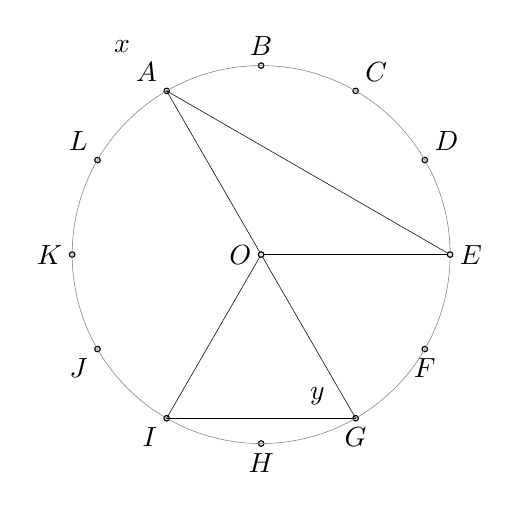
\begin{tikzpicture}[scale=0.8]
\tkzDefPoint(0,0){O}
\tkzDefPoint(3,0){E}
\foreach \i in {1,...,11}
	{
	\tkzDefPointBy[rotation = center O angle 30*\i](E) \tkzGetPoint{a\i}
	\tkzDrawPoint(a\i)
	}
\tkzDrawCircle(O,E)
\tkzDrawSegments(O,a4 O,E a4,E O,a8 a8,a10 a10,O)
\tkzLabelAngle[pos=1](E,a4,O){$x$}
\tkzLabelAngle[pos=0.7](O,a10,a8){$y$}
\tkzDrawPoints(O,E)
\tkzLabelPoint[left](O){$O$}
\tkzLabelPoint[right](E){$E$}
\tkzLabelPoint[above right](a1){$D$}
\tkzLabelPoint[above right](a2){$C$}
\tkzLabelPoint[above](a3){$B$}
\tkzLabelPoint[above left](a4){$A$}
\tkzLabelPoint[above left](a5){$L$}
\tkzLabelPoint[left](a6){$K$}
\tkzLabelPoint[below left](a7){$J$}
\tkzLabelPoint[below left](a8){$I$}
\tkzLabelPoint[below](a9){$H$}
\tkzLabelPoint(a10){$G$}
\tkzLabelPoint(a11){$F$}
\end{tikzpicture}
\end{center}
\end{frame}

\begin{frame}{Question 9}
\begin{quest}
George walks $1$ mile to school. He leaves home at the same time each day, walks at a steady speed of $3$ miles per hour, and arrives just as school begins. Today he was distracted by the pleasant weather and walked the first $\frac{1}{2}$ mile at a speed of only $2$ miles per hour. At how many miles per hour must George run the last $\frac{1}{2}$ mile in order to arrive just as school begins today?
\end{quest}
\end{frame}

\begin{frame}{Question 10}
\begin{quest}
A cube with 3-inch edges is to be constructed from 27 smaller cubes with 1-inch edges. Twenty-one of the cubes are colored red and 6 are colored white. If the 3-inch cube is constructed to have the smallest possible white surface area showing, what fraction of the surface area is white?
\end{quest}
\end{frame}

\end{document}


